\section{Trigonometric Functions}

\subsection{The Unit Circle}
\begin{frame}
    \frametitle{The Unit Circle}
    \begin{definition}
        The \textbf{unit circle} is the circle in the Cartesian plane with center at the origin and radius 1, defined by the equation:
        \[
        x^2 + y^2 = 1
        \]
    \end{definition}                                                                                                                                    
\end{frame}

\begin{frame}
    \frametitle{Radius corresponding to a positive angle}
    \centering
    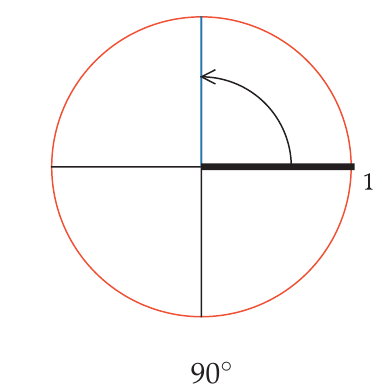
\includegraphics[scale=0.5]{/unit_circle/1.png}
\end{frame}

\begin{frame}
    \frametitle{Radius corresponding to a negative angle}
    \centering
    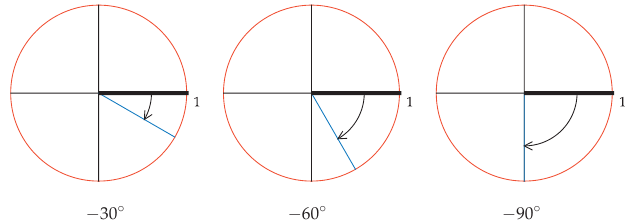
\includegraphics[scale=0.5]{/unit_circle/2.png}
\end{frame}

\begin{frame}
    \begin{block}{Positive and Negative Angles}
        \begin{itemize}
            \item Angle measurements for a radius on the unit circle are made from the positive horizontal axis.
            \item Positive angles correspond to moving counterclockwise from the positive horizontal axis.
            \item Negative angles correspond to moving clockwise from the positive horizontal axis.
        \end{itemize}
    \end{block}
\end{frame}

\begin{frame}
    \frametitle{Angles more than 360 degrees}
    \begin{block}{cyclic behaviour of angles}
        A radius of the unit circle corresponding to $\theta$ degrees also corresponds to $\theta + 360n$ degrees for every integer n.
    \end{block}
    \begin{figure}[h]    
        \centering
        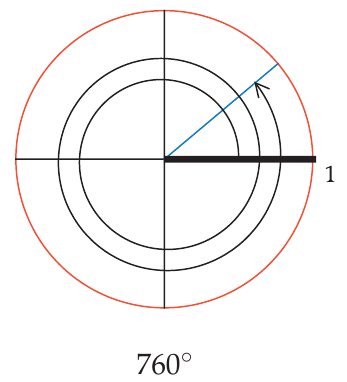
\includegraphics[scale=0.4]{/unit_circle/3.png}
    \end{figure}
\end{frame}

\begin{frame}
    \frametitle{Length of a Circular Arc}
    \begin{figure}
        \centering
        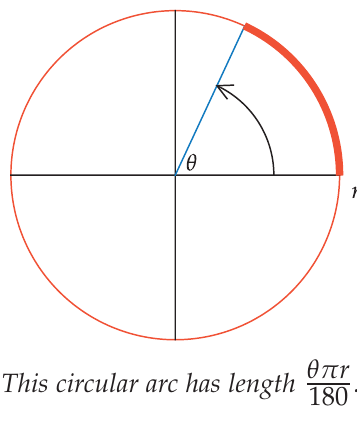
\includegraphics[scale=0.5]{/unit_circle/5.png}
    \end{figure}
    \[ 360^{\circ}   \rightarrow  2 \pi r \implies \theta^{\circ}  \rightarrow \frac{\theta}{360}.2\pi r  = \frac{\theta \pi r}{180}\] 
\end{frame}

\begin{frame}
    \frametitle{Radians}
    For example an ant moving around a unit circle would travel a distance of $2\pi$ radians when it completes one full rotation.
    \begin{block}{Radians}
        Radians are a unit of measurement for angles such that $2\pi$ radians correspond to a rotation through an entire circle.
    \end{block}
\end{frame}

\begin{frame}
    \frametitle{Radians}
    \begin{block}{Degree to Radians}
        \[ 360^{\circ} = 2 \pi \text{ radians} \]
        \[ \theta ^{\circ}  = \frac{\theta \pi}{180} \text{ radians} \]
    \end{block}
\end{frame}

\begin{frame}
    \frametitle{Arc Length}
    \begin{block}{length of a circular arc}
        If $0 < \theta \leq 2\pi$ , then a circular arc on the unit circle corresponding to $\theta$ radians has length $\theta$         
    \end{block}
\end{frame}

\begin{frame}
    \frametitle{Area of a Sector}
    \begin{block}{Area of a sector}
        A sector/slice with angle $\theta$ radians inside a circle with radius $r$ has area $\frac{1}{2} \theta r^{2}$ .
    \end{block}
    \begin{figure}[h]    
        \centering
        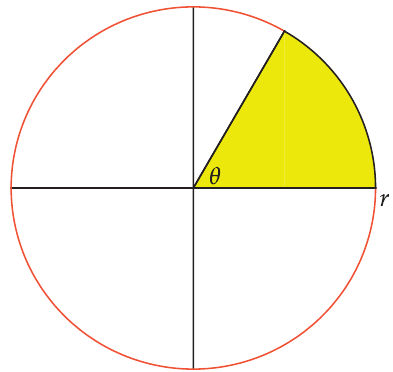
\includegraphics[scale=0.25]{unit_circle/6.png}
    \end{figure}
\end{frame}

\begin{frame}
    \frametitle{Note}
    \begin{block}{Note}
        If no unit is specified, angles are assumed to be in radians.
    \end{block}
\end{frame}

\begin{frame}
    \frametitle{Cosine and Sine}
    \begin{block}{Definitions}
        \begin{itemize}
            \item The \textbf{cosine} of an angle $\theta$ is the x-coordinate of the point on the unit circle corresponding to that angle.
            \item The \textbf{sine} of an angle $\theta$ is the y-coordinate of the point on the unit circle corresponding to that angle.
        \end{itemize}
    \end{block}     
    \begin{figure}[h]    
        \begin{minipage}[b]{0.8\textwidth}
            \centering
            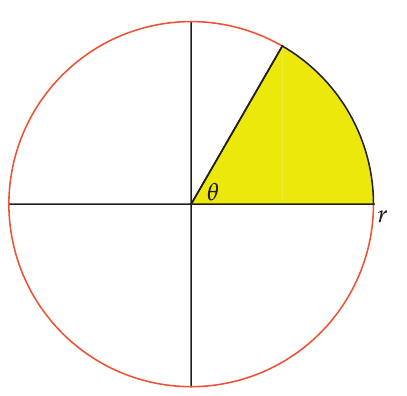
\includegraphics[scale=0.22]{unit_circle/7.png}
            \caption{sine and cosine}
        \end{minipage}
    \end{figure}
\end{frame}

\begin{frame}
    \frametitle{The Signs of Sine and Cosine} 
    \begin{figure}
        \centering
        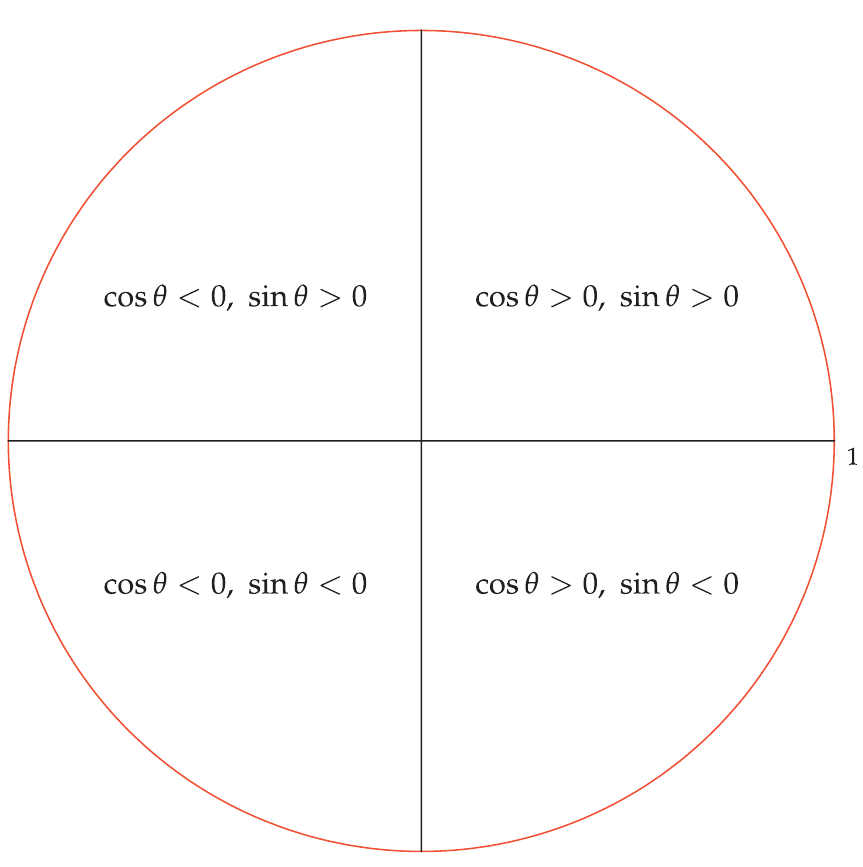
\includegraphics[scale=0.2]{unit_circle/8.png}
        \caption{Signs of sine and cosine in different quadrants}
    \end{figure}
\end{frame}

\begin{frame}
    \frametitle{Key Equation Connecting Sine and Cosine} 
    \begin{itemize}
        \item By definition cosine and sine are the x and y coordinates of a point on the unit circle.
        \item The equation of the unit circle is $x^2 + y^2 = 1$.
        \item Therefore, for any angle $\theta$,
    \end{itemize}
    \begin{block}{Key Identity}
        \[\cos^2(\theta) + \sin^2(\theta) = 1\]
    \end{block}
\end{frame}

\begin{frame}
    \frametitle{The limits of Sine and Cosine} 
    \begin{itemize}
        \item For each real number $\theta$, there is a radius of the unit circle corresponding to that angle.
        \item The co-ordinates of the end point of the radius are $(\cos(\theta), \sin(\theta))$.
        \item That is this function is defined for all real numbers because theta can take any real value. 
        \item The domain of sine and cosine is all real numbers. \(\mathbb{R}\) 
        \item For unit circle \( \cos \theta^{2} + \sin \theta^{2} = 1 \) 
        \item Because \( \cos \theta^{2} + \sin \theta^{2} = 1 \) for all \(\theta\), the range of both sine and cosine is limited to \([-1, 1]\).
    \end{itemize}
\end{frame}

\begin{frame}
    \frametitle{Domain and Range of Sine and Cosine}
    \begin{block}{Cosine and Sine are between -1 and 1}
        \[
        -1 \leq \cos(\theta) \leq 1 \quad \text{and} \quad -1 \leq \sin(\theta) \leq 1
        \] for all \(\theta \in \mathbb{R}\)
    \end{block}
    \begin{block}{Domain and Range}
        \begin{itemize}
            \item Domain of sine and cosine: \(\mathbb{R}\)
            \item Range of sine and cosine: \([-1, 1]\)
        \end{itemize}
    \end{block}
\end{frame}

\begin{frame}
    \frametitle{Tangent}
    \begin{block}{Definition of Tangent}
        The \textbf{tangent} of an angle $\theta$ is defined as the ratio of the sine to the cosine of that angle:
        \[\tan(\theta) = \frac{\sin(\theta)}{\cos(\theta)}\]   
        provided that \(\cos(\theta) \neq 0\).
    \end{block}
\end{frame}

\begin{frame}
    \frametitle{Tangent as Slope}
    \begin{figure}
        \centering
        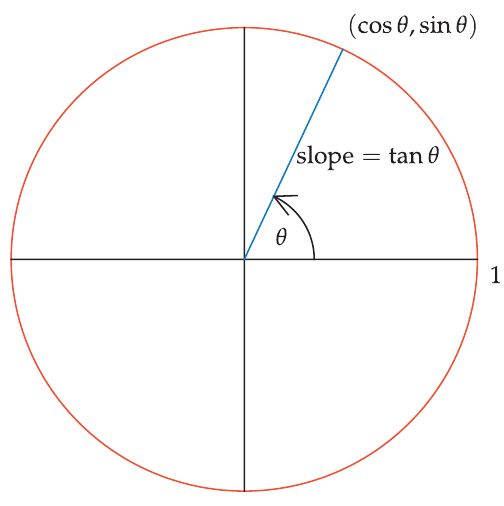
\includegraphics[scale=0.2]{unit_circle/9.png}
        \caption{Tangent as slope of the radius}
    \end{figure}
    \centering
    \[ 
        \text{Slope} = \frac{y_{2} - y_{1}}{x_{2} - x_{1}} = \frac{\sin(\theta) - 0}{\cos(\theta) - 0} = \tan(\theta)
    \]
    \(\tan \theta\) is the slope of the radius corresponding to angle \(\theta\) in the \textbf{unit circle}.
    \textbf{Note:} The slope of the radius applies to any circle, not just the unit circle.
\end{frame}

\begin{frame}
    \frametitle{Sign of Tangent}
    \begin{figure}
        \centering
        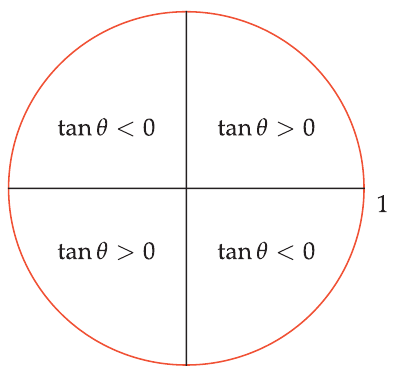
\includegraphics[scale=0.2]{unit_circle/10.png}
        \caption{Signs of tangent in different quadrants}
    \end{figure}
\end{frame}

\begin{frame}
    \frametitle{Radius of unit circle corresponding to a positive angle}
    \begin{figure}
        \centering
        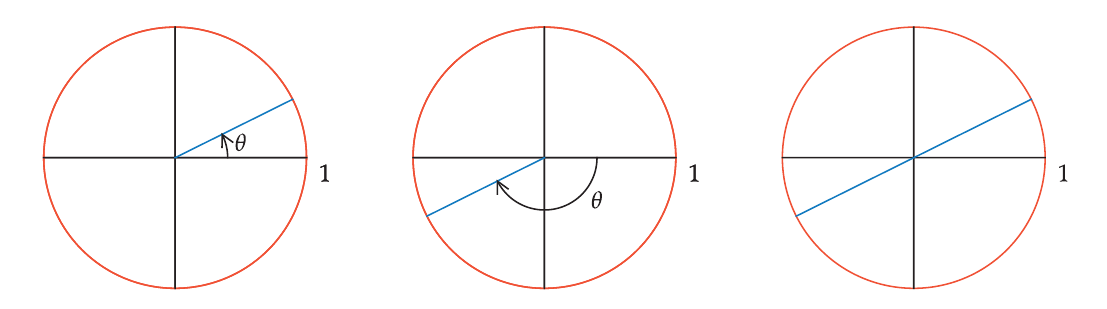
\includegraphics[scale=0.25]{unit_circle/11.png}
        \caption{Radius of unit circle corresponding to angle \(\theta\) such that \(\tan(\theta) = \frac{1}{2}\)}
    \end{figure}
\end{frame}

\begin{frame}
    \frametitle{Domain and Range of Tangent}
    \begin{itemize}
        \item Tangent is defined for all angles except those where \(\cos(\theta) = 0\), which occurs at odd multiples of \(\frac{\pi}{2}\).
        \item The tangent of an angle is the slope of the corresponding radius in the unit circle.
        \item Every real number is the slope of some radius in the unit circle. So range of tangent is all real numbers.
        \item The domain of tangent is all real numbers except odd multiples of \(\frac{\pi}{2}\):
        \[\text{Domain of } \tan(\theta) = \mathbb{R} \setminus \left\{ \theta \mid \theta = \frac{\pi}{2} + n\pi, n \in \mathbb{Z} \right\}\]
        \item The range of tangent is all real numbers:
        \[\text{Range of } \tan(\theta) = \mathbb{R}\]  
    \end{itemize}

\end{frame} 

\begin{frame}
    \frametitle{Graphing Tangent: Tangent near \(\frac{\pi}{2}\)}
    \begin{figure}
        \centering
        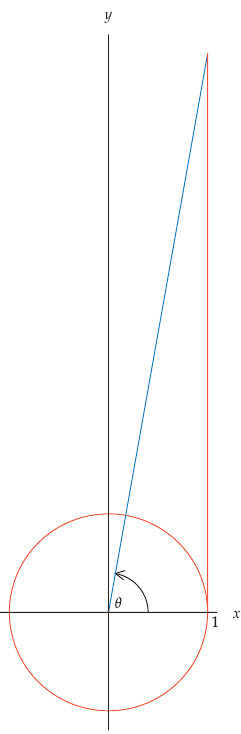
\includegraphics[scale=0.28]{/unit_circle/12.png}
    \end{figure}
\end{frame}

\subsection{Trigonometry in Right Triangles}
\begin{frame}
    \frametitle{Right Triangle Definitions}
    For \(0<\theta<\frac{\pi}{2}\) in a right triangle:
    \begin{itemize}
        \item In a right triangle, the side opposite the right angle is the \textbf{hypotenuse}.
        \item The other two sides are referred to as the \textbf{adjacent} and \textbf{opposite} sides, depending on the angle of interest.
    \end{itemize}
\end{frame}
\begin{frame}
    \frametitle{Right Triangles}
    \begin{figure}
        \centering
        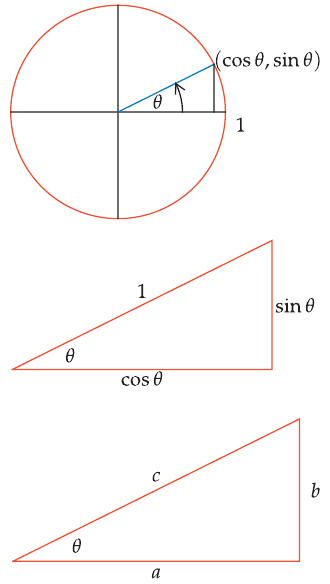
\includegraphics[scale=0.3]{/unit_circle/13.png}
    \end{figure}
\end{frame}

\begin{frame}
    \frametitle{SOH-CAH-TOA}
    \begin{itemize}
        \item \textbf{SOH}: \(\sin(\theta) = \frac{\text{opposite}}{\text{hypotenuse}}\)
        \item \textbf{CAH}: \(\cos(\theta) = \frac{\text{adjacent}}{\text{hypotenuse}}\)
        \item \textbf{TOA}: \(\tan(\theta) = \frac{\text{opposite}}{\text{adjacent}}\)
    \end{itemize}
\end{frame}

\begin{frame}
    \frametitle{Trigonometric Identities}
   
    \begin{block}{Trigonometric Identities}
        \begin{itemize}
            \item \(\sin^2(\theta) + \cos^2(\theta) = 1\)
            \item \(\tan(\theta) = \frac{\sin(\theta)}{\cos(\theta)}\)
            \item \(\cot(\theta) = \frac{1}{\tan(\theta)} = \frac{\cos(\theta)}{\sin(\theta)}\)
            \item \(\sec(\theta) = \frac{1}{\cos(\theta)}\)
            \item \(\csc(\theta) = \frac{1}{\sin(\theta)}\)
            \item 
        \end{itemize}
    \end{block}
\end{frame}

\begin{frame}
\frametitle{Trigonometric Identities For Negative Angles}
\begin{columns}
    \begin{column}{0.5\textwidth}
        \begin{figure}
            \centering
            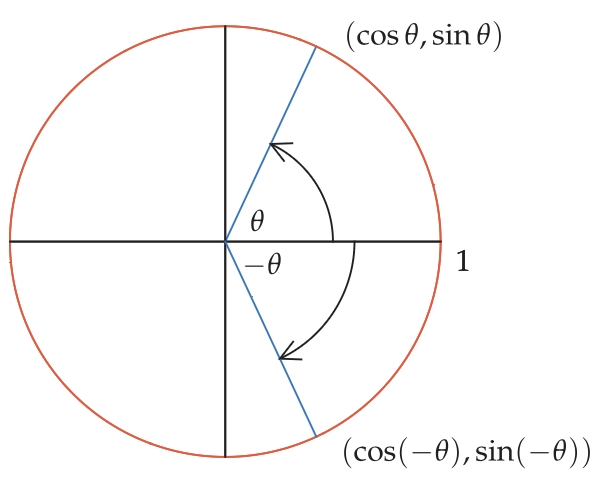
\includegraphics[scale=0.4]{/unit_circle/14.png}
            \caption{Trigonometric identities in a right triangle}
        \end{figure}
    \end{column}
    \begin{column}{0.5\textwidth}
        \begin{block}{}
            \begin{itemize}
                \item \(\sin(-\theta) = -\sin(\theta)\)
                \item \(\cos(-\theta) = \cos(\theta)\)
                \item \(\tan(-\theta) = -\tan(\theta)\)
            \end{itemize}
        \end{block}
    \end{column}
\end{columns}
\end{frame} 

\begin{frame}
    \frametitle{Even and Odd Trigonometric Functions}
    \begin{itemize}
        \item \textbf{Even Functions:} \(\cos(-\theta) = \cos(\theta)\) 
        \item \textbf{Odd Functions:} \(\sin(-\theta) = -\sin(\theta)\), \(\tan(-\theta) = -\tan(\theta) \)
    \end{itemize}   
\end{frame}

\begin{frame}
    \frametitle{Trigonometric Identities with Right Triangles}
    \begin{figure}
        \centering
        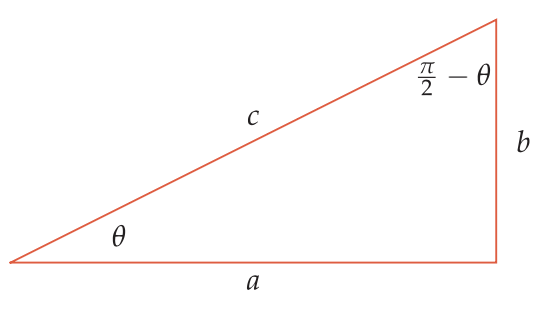
\includegraphics[scale=0.4]{/unit_circle/15.png}
        \caption{Trigonometric identities in a right triangle}
    \end{figure}

    \begin{itemize}
        \item  \(\sin(\pi/2 - \theta) = \cos(\theta)\)
        \item \(\cos(\pi/2 - \theta) = \sin(\theta)\)
        \item \(\tan(\pi/2 - \theta) = \frac{1}{\tan(\theta)} = \cot(\theta)\)
    \end{itemize}
\end{frame}

\begin{frame}
    \frametitle{Trigonometric Identities involving multiples of \(\pi\)}
    \begin{figure}
        \centering
        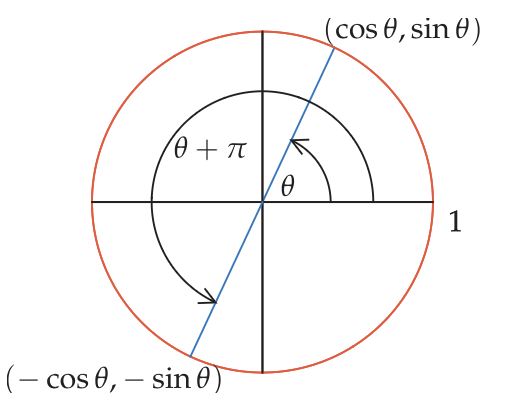
\includegraphics[scale=0.5]{/unit_circle/16.png}
        \caption{Trigonometric identities involving multiples of \(\pi\)}
    \end{figure}
    \begin{itemize}
        \item \(\sin(n\pi + \theta) = (-1)^n \sin(\theta)\)
        \item \(\cos(n\pi + \theta) = (-1)^n \cos(\theta)\)
        \item \(\tan(n\pi + \theta) = \tan(\theta)\)
    \end{itemize}
    For example, if \(n\) is even, \(\sin(n\pi + \theta) = \sin(\theta)\) and if \(n\) is odd, \(\sin(n\pi + \theta) = -\sin(\theta)\). 
\end{frame}

\section{Trigonometric Algebra and Geometry}
\subsection{Inverse Trigonometric Functions}
\begin{frame}
    \frametitle{The Arccosine Function}
    \begin{itemize}
        \item A function is called one-to-one if it maps distinct inputs to distinct outputs.
        \item The \textbf{cosine function} whose domain is entire real line \(\mathbb{R}\) is not one-to-one because it takes the same value for different angles. For example, \(\cos(0) = \cos(2\pi) = 1\).
        \item Thus the cosine function is not invertible. It fails in horixontal line test
        \item To make it invertible, we restrict the domain to \([0, \pi]\) where it is one-to-one.
    \end{itemize}
\end{frame}

\begin{frame}
    \frametitle{The Arccosine Function}
    \begin{figure}
        \centering
        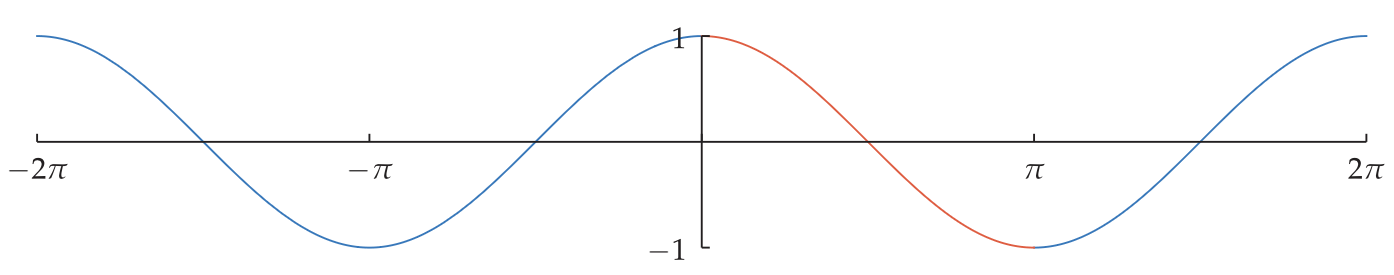
\includegraphics[scale=0.3]{/unit_circle/18.png}
        \caption{Graph of the cosine function restricted to \([0, \pi]\)}
    \end{figure}
    \begin{block}{The Arccosine Function}
        The \textbf{arccosine function} is the inverse of the cosine function restricted to the interval \([0, \pi]\):
        \[
        \arccos(x) = \theta \quad \text{if and only if} \quad x = \cos(\theta) \text{ for } 0 \leq \theta \leq \pi
        \]
    \end{block}
\end{frame}

\begin{frame}
\frametitle{The domain and range of the Arccosine Function}
\begin{itemize}
    \item \textbf{Domain:} The domain of the arccosine function is \([-1, 1]\) because the cosine function takes values in this interval.
    \item \textbf{Range:} The range of the arccosine function is \([0, \pi]\) because it outputs angles in this interval.
\end{itemize}       
\end{frame}

\begin{frame}
    \frametitle{The Arcsine Function}
    \begin{figure}
        \centering
        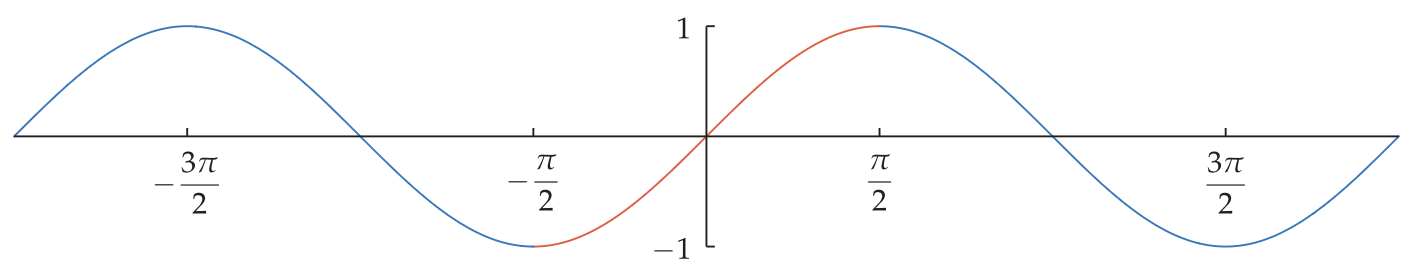
\includegraphics[scale=0.3]{/unit_circle/19.png}
        \caption{Graph of the sine function restricted to \([- \frac{\pi}{2}, \frac{\pi}{2}]\)}
    \end{figure}
    \begin{itemize}
        \item The \textbf{sine function} is also not one-to-one over the entire real line because it takes the same value for different angles. For example, \(\sin(0) = \sin(\pi) = 0\).
        \item To make it invertible, we restrict the domain to \([- \frac{\pi}{2}, \frac{\pi}{2}]\) where it is one-to-one.
    \end{itemize}
\end{frame}

\begin{frame}
    \frametitle{The Arcsine Function}
    \begin{block}{The Arcsine Function}
        The \textbf{arcsine function} is the inverse of the sine function restricted to the interval \([- \frac{\pi}{2}, \frac{\pi}{2}]\):
        \[
        \arcsin(x) = \theta \quad \text{if and only if} \quad x = \sin(\theta) \text{ for } -\frac{\pi}{2} \leq \theta \leq \frac{\pi}{2}
        \]
    \end{block}
\end{frame}

\begin{frame}
    \frametitle{The domain and range of the Arcsine Function}
    \begin{itemize}
        \item \textbf{Domain:} The domain of the arcsine function is \([-1, 1]\) because the sine function takes values in this interval.
        \item \textbf{Range:} The range of the arcsine function is \([- \frac{\pi}{2}, \frac{\pi}{2}]\) because it outputs angles in this interval.
    \end{itemize}       
\end{frame}


    \begin{frame}
    \frametitle{The Arctangent Function}
    \begin{block}{The Arctangent Function}
    \begin{itemize}
        \item The \textbf{tangent function} is not one-to-one over the entire real line because it takes the same value for different angles. For example, \(\tan(0) = \tan(\pi) = 0\).
        \item To make it invertible, we restrict the domain to \((- \frac{\pi}{2}, \frac{\pi}{2})\) where it is one-to-one.
    \end{itemize}
    \end{block}
\end{frame}

\begin{frame}
    \frametitle{The Arctangent Function}
    \begin{figure}
        \centering
        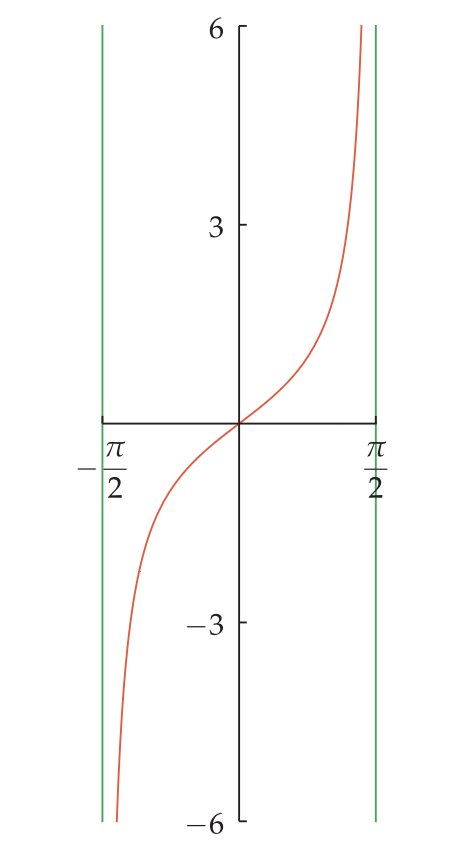
\includegraphics[scale=0.4]{/unit_circle/20.png}
        \caption{Graph of the tangent function restricted to \((- \frac{\pi}{2}, \frac{\pi}{2})\)}
    \end{figure}
\end{frame}

\begin{frame}
    \frametitle{The Arctangent Function}
    \begin{block}{The Arctangent Function}
        The \textbf{arctangent function} is the inverse of the tangent function restricted to the interval \((- \frac{\pi}{2}, \frac{\pi}{2})\):
        \[
        \arctan(x) = \theta \quad \text{if and only if} \quad x = \tan(\theta) \text{ for } -\frac{\pi}{2} < \theta < \frac{\pi}{2}
        \]
    \end{block}
\end{frame}

\begin{frame}
    \frametitle{Inverse Trigonometric Identities}
    \begin{itemize}
        \item \(\arccos(\cos(x)) = x\) for \(0 \leq x \leq \pi\)
        \item \(\arcsin(\sin(x)) = x\) for \(-\frac{\pi}{2} \leq x \leq \frac{\pi}{2}\)
        \item \(\arctan(\tan(x)) = x\) for \(-\frac{\pi}{2} < x < \frac{\pi}{2}\)
    \end{itemize}
    \begin{block}{Note}
        \begin{itemize}
            \item The inverse trigonometric functions return angles in their respective ranges.
            \item For example, \(\arccos(0.5) = \frac{\pi}{3}\) because \(\cos(\frac{\pi}{3}) = 0.5\) and \(\frac{\pi}{3}\) is in the range of the arccosine function.
            \item Similarly, \(\arcsin(0.5) = \frac{\pi}{6}\) because \(\sin(\frac{\pi}{6}) = 0.5\) and \(\frac{\pi}{6}\) is in the range of the arcsine function.
            \item \(\arctan(1) = \frac{\pi}{4}\) because \(\tan(\frac{\pi}{4}) = 1\) and \(\frac{\pi}{4}\) is in the range of the arctangent function.
        \end{itemize}
    \end{block} 
\end{frame}

% Add this line to your preamble if not already present:
% \usepackage{enumitem}

\begin{frame}{Inverse of $f(x)=3+4\cos x$}
  \begin{block}{Problem}
    Suppose $f(x)=3+4\cos x$, where the domain of $f$ is $[0,\pi]$.
    \begin{enumerate}[]
      \item Find a formula for $f^{-1}(y)$.
      \item What is the domain of $f^{-1}$?
      \item What is the range of $f^{-1}$?
    \end{enumerate}
  \end{block}
  \begin{block}{Solution}
    \begin{itemize}
      \item $f^{-1}(y)=\arccos\left(\frac{y-3}{4}\right)$.
      \item $\operatorname{dom}(f^{-1})=[-1,7]$.
      \item $\operatorname{range}(f^{-1})=[0,\pi]$.
    \end{itemize}
  \end{block}
\end{frame}


\begin{frame}
    \frametitle{Find the \(\arccos(-t)\)}
    \begin{figure}
        \centering
        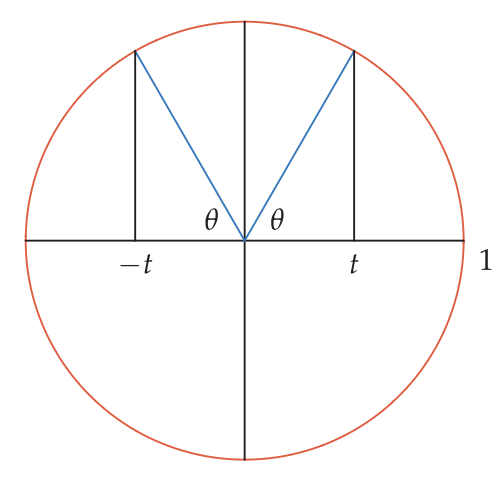
\includegraphics[scale=0.4]{/unit_circle/21.png}
        \caption{Graph of the arccosine function}
    \end{figure}
    \textbf{Solution:} 
    \[ x = -t \implies \arccos(-t) = \pi - \arccos(t) \] 
\end{frame}

\begin{frame}
\frametitle{Find the \(\arcsin(t)\)}
\begin{figure}
    \centering
    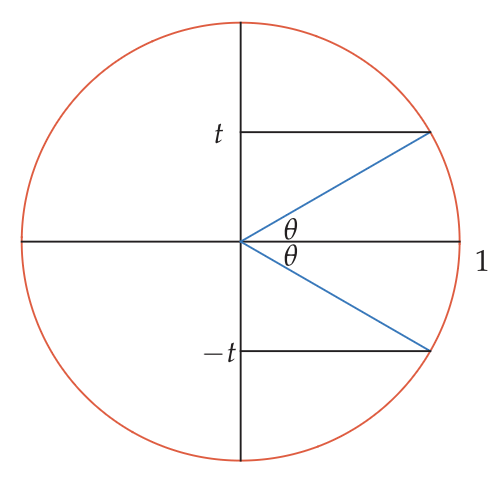
\includegraphics[scale=0.4]{/unit_circle/22.png}
    \caption{Graph of the arcsine function}
\end{figure}
\textbf{Solution:} 
\[ y = -t \implies \arcsin(-t) = -\sin(\theta) \] 
\end{frame}

\begin{frame}
    \frametitle{Inverse trigonometric identities for \(-t\)}
    \begin{itemize}
        \item \( \cos^{-1}(-t) = \pi - \cos^{-1}(t) \)
        \item \( \sin^{-1}(-t) = - \sin^{-1}(t) \)  
        \item \( \tan^{-1}(-t) = -\tan^{-1}(t) \)
    \end{itemize}
\end{frame}

\begin{frame}
    \frametitle{Find the \(\arctan(-t)\)}
    \begin{figure}
        \centering
        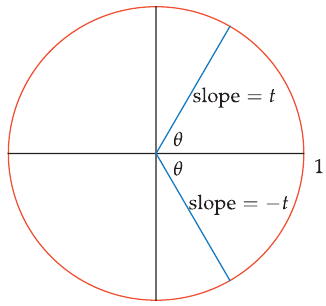
\includegraphics[scale=0.4]{/unit_circle/23.png}
        \caption{Graph of the arctangent function}
    \end{figure}
\end{frame}

\begin{frame}
    \frametitle{arcsin plus arccosine}
    \begin{block}{Identity}
        \[ \arcsin(t) + \arccos(t) = \frac{\pi}{2} \]
    \end{block}
    \begin{itemize}
        \item This identity holds for all \(t\) in the domain of both functions, which is \([-1, 1]\).
        \item The identity reflects the complementary nature of the sine and cosine functions.
        \item Geometrically, it represents the relationship between the angles in a right triangle where one angle is \(\arcsin(t)\) and the other is \(\arccos(t)\).
    \end{itemize}   
\end{frame}


\begin{frame}
    \frametitle{arcsin + arccosine}
    \begin{figure}
        \centering
        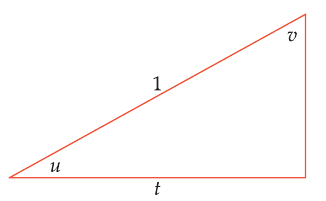
\includegraphics[scale=0.4]{/unit_circle/24.png}
        \caption{right angle triangle involving arcsine and arccosine functions}      
    \end{figure}
\end{frame}

\subsection{Trignometry to Compute Area}

\begin{frame}
    \frametitle{Area of a Triangle}
    \begin{block}{Area of a Triangle}
        The area \(A\) of a triangle with base \(b\) and height \(h\) is given by:
        \[
        A = \frac{1}{2} b h = \frac{1}{2} b c \sin(\theta)
        \]
        where \(\theta\) is the angle between the two sides of length \(b\) and \(c\).
    \end{block}
    \begin{figure}
        \centering
        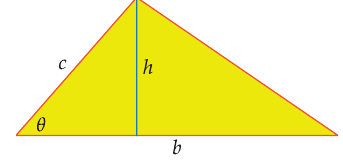
\includegraphics[scale=0.4]{/unit_circle/25.png}
        \caption{Area of a triangle using sine function}
    \end{figure}
\end{frame}

\begin{frame}
    \frametitle{Ambiguous Angles}
    \begin{figure}
        \centering
        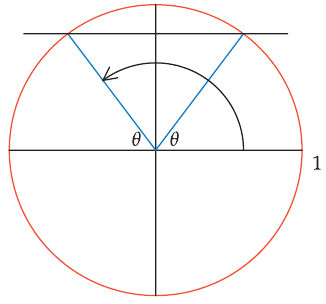
\includegraphics[scale=0.3]{/unit_circle/26.png}
        \caption{\(\sin(\pi - \theta) = \sin(\theta)\)}
    \end{figure}
    \begin{itemize}
        \item  \(A = \frac{1}{2} b c \sin(\theta) \implies \theta = \arcsin\left(\frac{2A}{bc}\right) \)
        \item Assume \( \frac{2A}{bc} = \frac{1}{2} \) 
        \item Then \( \theta = \arcsin\left(\frac{1}{2}\right) = \frac{\pi}{6} \) or \( \frac{5\pi}{6} \)
        \item That is given any number \(t \in [-1,1]\) there are two possible angles \(\theta\) that satisfy the equation.
        \item \(\sin (\pi - \theta) = \sin(-(\theta - \pi )) = - \sin(\theta - \pi) = -(-\sin \theta) = \sin \theta \)
    \end{itemize}
    \end{frame}

    \begin{frame}
        \frametitle{Area of a parallelogram}
        \begin{block}{Area of a Parallelogram}
            The area \(A\) of a parallelogram with base \(b\) and height \(h\) is given by:
            \[
            A = b h
            \]
            Alternatively, if we know the lengths of two sides \(a\) and \(b\) and the angle \(\theta\) between them, we can use:
            \[
            A =  bc \sin(\theta)
            \]
        \end{block}
        \begin{figure}
            \centering
            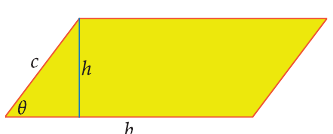
\includegraphics[scale=0.3]{/unit_circle/27.png}
            \caption{Area of a parallelogram using sine function}
        \end{figure}
    \end{frame}

    \begin{frame}
        \frametitle{Area of Polygon}
        \begin{columns}
            \begin{column}{0.5\textwidth}
                \begin{itemize}
                    \item Area of one triangle = \(\frac{1}{2} \cdot 1 \cdot 1 \sin(\frac{2\pi}{8})\)
                    \item Total Area of polygon = \(8 \cdot \frac{1}{2} \cdot 1 \cdot 1 \sin(\frac{2\pi}{8})\)
                    \item Total area of regular polygon with \(n\) sides = \(\frac{n}{2} \cdot 1 \cdot 1 \sin(\frac{2\pi}{n})\)
                \end{itemize}
            \end{column}
            \begin{column}{0.5\textwidth}
                \begin{figure}
                    \centering
                    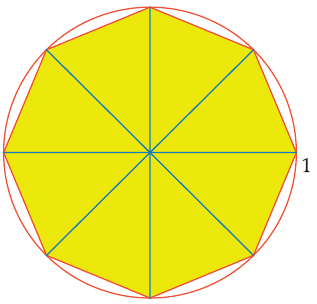
\includegraphics[scale=0.3]{/unit_circle/28.png}
                    \caption{Area of a regular polygon using sine function}
                \end{figure}
            \end{column}
        \end{columns}
    \end{frame}
    
    \begin{frame}
        \frametitle{Example: Area of a Regular Pentagon}
    \begin{columns}
        \begin{column}{0.5\textwidth}
            Each side of the Pentagon that houses the U.S. Department of Defense has a length of 921 feet.
            \begin{figure}
                \centering
                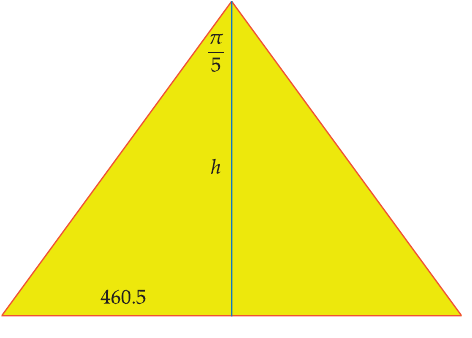
\includegraphics[scale=0.3]{/unit_circle/29.png}
                \caption{Area of a regular pentagon}
            \end{figure}
        \end{column}
        \begin{column}{0.5\textwidth}
            \begin{block}{Solution}
                \begin{itemize}
                    \item \(h = \frac{460.5}{\tan (\frac{\pi}{5})}\) 
                    \item \(\frac{1}{2} \cdot 921 \cdot h\)
                    \item \(5 \cdot \frac{1}{2} \cdot 921 \cdot h\)
                \end{itemize}
            \end{block}
        \end{column}
    \end{columns}
    \end{frame}

    \begin{frame}
    \frametitle{Trignometric Approximation}

    \begin{table}[h]
        \centering
        \begin{tabular}{|c|c|c|}
            \hline
            $q$ & $\sin q$ & $\tan q$ \\
            \hline
            0.5 & 0.47943 & 0.54630 \\
            0.05 & 0.04998 & 0.05004 \\
            0.005 & 0.00499998 & 0.00500004 \\
            0.0005 & 0.00049999998 & 0.00050000004 \\
            0.00005 & 0.00004999999998 & 0.00005000000004 \\
            \hline
        \end{tabular}
        \caption{Values of $\sin q$ and $\tan q$ for small $q$}
    \end{table}

    \begin{block}{Approximation of \(\sin \theta\) and \(\tan \theta\)}
        If \(| \theta | << 1\), then \(\sin \theta \approx \theta\) and \(\tan \theta \approx \theta\).
    \end{block}
    \begin{block}{Note}
        This approximation is applicable only for radians. For small angles in degrees, the approximation is not valid.
    \end{block}

    \end{frame}

    \begin{frame}
        \frametitle{\(\sin \theta\) for small angles}
        \begin{columns}
            \begin{column}{0.5\textwidth}
                \begin{figure}
                    \centering
                    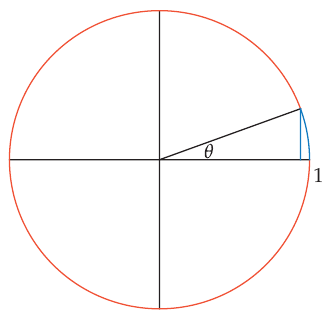
\includegraphics[scale=0.4]{/unit_circle/30.png}
                    \caption{Graph of \(\sin \theta\) for small angles}
                \end{figure}
            \end{column}
            \begin{column}{0.5\textwidth}
                \begin{itemize}
                    \item The blue vertical line and the blue circular arc have nearly the same length if \(|\theta| << 1\).
                    \item The blue vertical line represents \(\sin \theta\), and the blue circular arc represents \(\theta\).
                    \item From the figure, we see that \(\sin \theta < \theta\) for small angles.
                \end{itemize}
            \end{column}
        \end{columns}
        \end{frame}

    \begin{frame}
        \frametitle{\(\tan \theta\) for small angles}
        \begin{columns}
            \begin{column}{0.5\textwidth}
                \begin{figure}
                    \centering
                    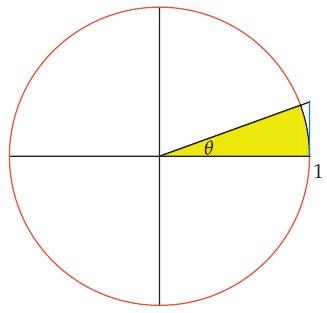
\includegraphics[scale=0.4]{/unit_circle/31.png}
                    \caption{Graph of \(\tan \theta\) for small angles}
                \end{figure}
            \end{column}
            \begin{column}{0.5\textwidth}
                \begin{itemize}
                    \item The yellow region has the area = \(\frac{1}{2} \cdot \theta\)  
                    \item The blue vertical line has the length \(\tan \theta\) 
                    \item The right triangle which has the base 1 and height \(\tan \theta\) has area = \(\frac{1}{2} \cdot 1 \cdot \tan \theta\)
                    \item As the yellow region lies inside the triangle, we have \(\frac{1}{2} \cdot \theta < \frac{1}{2} \cdot 1 \cdot \tan \theta\)  
                    \item Thus \(\theta < \tan \theta\)     
                \end{itemize}
            \end{column}
        \end{columns}
    \end{frame}

    \begin{frame}
    \frametitle{Trignometric Inequality}
    \begin{block}{Inequality of \(\sin \theta\) and \(\tan \theta\)}
        If \( 0 < \theta < \frac{\pi}{2} \), then \(\sin \theta < \theta < \tan \theta \).
    \end{block}
    \begin{displaymath}
        \theta < \tan \theta \implies \theta < \frac{\sin \theta}{\cos \theta} \implies \theta \cos \theta < \sin \theta \implies \cos \theta < \frac{\sin \theta}{\theta}
    \end{displaymath}
    \begin{displaymath}
        \sin \theta < \theta \implies \frac{\sin \theta}{\theta} < 1
    \end{displaymath}
    \begin{block}{Inequality for \( \frac{\sin \theta}{\theta} \)}
        If \( 0 < |\theta| < \frac{\pi}{2} \), then
        \[ \cos \theta <  \frac{\sin \theta}{\theta} < 1 \]
    \end{block}
    \end{frame}

    \begin{frame}
        \frametitle{Approximations}
        \begin{block}{\( \frac{\sin \theta}{\theta} \)}
            As \( \theta \) approaches 0, \( \frac{\sin \theta}{\theta} \) approaches 1.
        \end{block}
        \begin{block}{\(  \cos \theta \)}
            As \( |\theta| \) is small, \( \cos \theta \) approaches to  \(1 - \frac{\theta^2}{2} \)

        \end{block}


    \end{frame}
